\hypertarget{a00009}{
\section{Dokumentacja pliku /home/pawel/Dokumenty/Uczelnia/grupappz/Source/Ass8-server/include/md5/md5.cpp}
\label{a00009}\index{/home/pawel/Dokumenty/Uczelnia/grupappz/Source/Ass8-server/include/md5/md5.cpp@{/home/pawel/Dokumenty/Uczelnia/grupappz/Source/Ass8-server/include/md5/md5.cpp}}
}
{\tt \#include \char`\"{}md5.h\char`\"{}}\par


Wykres zależności załączania dla md5.cpp:\nopagebreak
\begin{figure}[H]
\begin{center}
\leavevmode
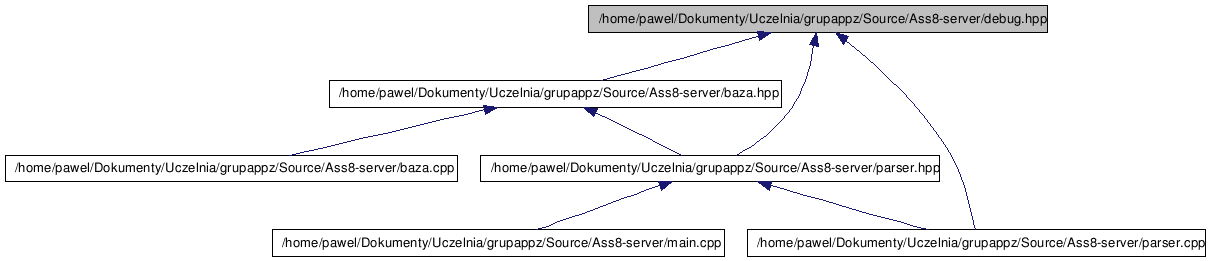
\includegraphics[width=218pt]{a00038}
\end{center}
\end{figure}
\subsection*{Definicje}
\begin{CompactItemize}
\item 
\#define \hyperlink{a00009_51398c0e5541164ad4d6615880073305}{S11}~7
\item 
\#define \hyperlink{a00009_1ec499cd0e54ecc28c2ac2afea5b038e}{S12}~12
\item 
\#define \hyperlink{a00009_aeec90429105fb54d853dd4fc7027a54}{S13}~17
\item 
\#define \hyperlink{a00009_78342b0ccde2ed12fdf19a113cc266cf}{S14}~22
\item 
\#define \hyperlink{a00009_b6d5354f647a0e7592a1f051fc8377b2}{S21}~5
\item 
\#define \hyperlink{a00009_ddad30455da936bc1879ee9c72b46d59}{S22}~9
\item 
\#define \hyperlink{a00009_6321a8b29628936f76e9e78cf5bda95f}{S23}~14
\item 
\#define \hyperlink{a00009_0c09eb77d30a0d5f9154914147b86c20}{S24}~20
\item 
\#define \hyperlink{a00009_ef26590f8a880ee6f4a158168defcd89}{S31}~4
\item 
\#define \hyperlink{a00009_1d512424dd8a91e0a5bcc98563f33914}{S32}~11
\item 
\#define \hyperlink{a00009_1c854214533f6220e859b0063196abb3}{S33}~16
\item 
\#define \hyperlink{a00009_f6472be1d535970afee8e5266a74aa07}{S34}~23
\item 
\#define \hyperlink{a00009_b674ba129e588da55d1d494e1cf3c15e}{S41}~6
\item 
\#define \hyperlink{a00009_268ef1a49114a94b931cc6b313e3cd1b}{S42}~10
\item 
\#define \hyperlink{a00009_5aaa7121f39650d472746942ca68f959}{S43}~15
\item 
\#define \hyperlink{a00009_6a3989af72b55d169bd73a66f8620aae}{S44}~21
\item 
\#define \hyperlink{a00009_96d73bbd7af15cb1fc38c3f4a3bd82e9}{F}(x, y, z)~(((x) \& (y)) $|$ (($\sim$x) \& (z)))
\item 
\#define \hyperlink{a00009_d96b7cf3182ce2ba85e5a7a93b12c441}{G}(x, y, z)~(((x) \& (z)) $|$ ((y) \& ($\sim$z)))
\item 
\#define \hyperlink{a00009_e42219072d798876e6b08e6b78614ff6}{H}(x, y, z)~((x) $^\wedge$ (y) $^\wedge$ (z))
\item 
\#define \hyperlink{a00009_c0eafdc9ee161b71e7af98af736952fd}{I}(x, y, z)~((y) $^\wedge$ ((x) $|$ ($\sim$z)))
\item 
\#define \hyperlink{a00009_7417fd4e875360c0533fa5b412cdab49}{ROTATE\_\-LEFT}(x, n)~(((x) $<$$<$ (n)) $|$ ((x) $>$$>$ (32-(n))))
\item 
\#define \hyperlink{a00009_0a143972cb6c4fe16f0ffa8a3d41ebf3}{FF}(a, b, c, d, x, s, ac)
\item 
\#define \hyperlink{a00009_685f32faa2a66e743850b990a13b8bfa}{GG}(a, b, c, d, x, s, ac)
\item 
\#define \hyperlink{a00009_8b9f1c4778df01ef970b87dbe5541dc5}{HH}(a, b, c, d, x, s, ac)
\item 
\#define \hyperlink{a00009_d26626e5efb37b2dadef4e88e35e4329}{II}(a, b, c, d, x, s, ac)
\end{CompactItemize}


\subsection{Dokumentacja definicji}
\hypertarget{a00009_96d73bbd7af15cb1fc38c3f4a3bd82e9}{
\index{md5.cpp@{md5.cpp}!F@{F}}
\index{F@{F}!md5.cpp@{md5.cpp}}
\subsubsection[{F}]{\setlength{\rightskip}{0pt plus 5cm}\#define F(x, \/  y, \/  z)~(((x) \& (y)) $|$ (($\sim$x) \& (z)))}}
\label{a00009_96d73bbd7af15cb1fc38c3f4a3bd82e9}




Definicja w linii 62 pliku md5.cpp.\hypertarget{a00009_0a143972cb6c4fe16f0ffa8a3d41ebf3}{
\index{md5.cpp@{md5.cpp}!FF@{FF}}
\index{FF@{FF}!md5.cpp@{md5.cpp}}
\subsubsection[{FF}]{\setlength{\rightskip}{0pt plus 5cm}\#define FF(a, \/  b, \/  c, \/  d, \/  x, \/  s, \/  ac)}}
\label{a00009_0a143972cb6c4fe16f0ffa8a3d41ebf3}


\textbf{Wartość:}

\begin{Code}\begin{verbatim}{ \
 (a) += F ((b), (c), (d)) + (x) + (unsigned long int)(ac); \
 (a) = ROTATE_LEFT ((a), (s)); \
 (a) += (b); \
  }
\end{verbatim}
\end{Code}


Definicja w linii 75 pliku md5.cpp.\hypertarget{a00009_d96b7cf3182ce2ba85e5a7a93b12c441}{
\index{md5.cpp@{md5.cpp}!G@{G}}
\index{G@{G}!md5.cpp@{md5.cpp}}
\subsubsection[{G}]{\setlength{\rightskip}{0pt plus 5cm}\#define G(x, \/  y, \/  z)~(((x) \& (z)) $|$ ((y) \& ($\sim$z)))}}
\label{a00009_d96b7cf3182ce2ba85e5a7a93b12c441}




Definicja w linii 63 pliku md5.cpp.\hypertarget{a00009_685f32faa2a66e743850b990a13b8bfa}{
\index{md5.cpp@{md5.cpp}!GG@{GG}}
\index{GG@{GG}!md5.cpp@{md5.cpp}}
\subsubsection[{GG}]{\setlength{\rightskip}{0pt plus 5cm}\#define GG(a, \/  b, \/  c, \/  d, \/  x, \/  s, \/  ac)}}
\label{a00009_685f32faa2a66e743850b990a13b8bfa}


\textbf{Wartość:}

\begin{Code}\begin{verbatim}{ \
 (a) += G ((b), (c), (d)) + (x) + (unsigned long int)(ac); \
 (a) = ROTATE_LEFT ((a), (s)); \
 (a) += (b); \
  }
\end{verbatim}
\end{Code}


Definicja w linii 81 pliku md5.cpp.\hypertarget{a00009_e42219072d798876e6b08e6b78614ff6}{
\index{md5.cpp@{md5.cpp}!H@{H}}
\index{H@{H}!md5.cpp@{md5.cpp}}
\subsubsection[{H}]{\setlength{\rightskip}{0pt plus 5cm}\#define H(x, \/  y, \/  z)~((x) $^\wedge$ (y) $^\wedge$ (z))}}
\label{a00009_e42219072d798876e6b08e6b78614ff6}




Definicja w linii 64 pliku md5.cpp.\hypertarget{a00009_8b9f1c4778df01ef970b87dbe5541dc5}{
\index{md5.cpp@{md5.cpp}!HH@{HH}}
\index{HH@{HH}!md5.cpp@{md5.cpp}}
\subsubsection[{HH}]{\setlength{\rightskip}{0pt plus 5cm}\#define HH(a, \/  b, \/  c, \/  d, \/  x, \/  s, \/  ac)}}
\label{a00009_8b9f1c4778df01ef970b87dbe5541dc5}


\textbf{Wartość:}

\begin{Code}\begin{verbatim}{ \
 (a) += H ((b), (c), (d)) + (x) + (unsigned long int)(ac); \
 (a) = ROTATE_LEFT ((a), (s)); \
 (a) += (b); \
  }
\end{verbatim}
\end{Code}


Definicja w linii 86 pliku md5.cpp.\hypertarget{a00009_c0eafdc9ee161b71e7af98af736952fd}{
\index{md5.cpp@{md5.cpp}!I@{I}}
\index{I@{I}!md5.cpp@{md5.cpp}}
\subsubsection[{I}]{\setlength{\rightskip}{0pt plus 5cm}\#define I(x, \/  y, \/  z)~((y) $^\wedge$ ((x) $|$ ($\sim$z)))}}
\label{a00009_c0eafdc9ee161b71e7af98af736952fd}




Definicja w linii 65 pliku md5.cpp.\hypertarget{a00009_d26626e5efb37b2dadef4e88e35e4329}{
\index{md5.cpp@{md5.cpp}!II@{II}}
\index{II@{II}!md5.cpp@{md5.cpp}}
\subsubsection[{II}]{\setlength{\rightskip}{0pt plus 5cm}\#define II(a, \/  b, \/  c, \/  d, \/  x, \/  s, \/  ac)}}
\label{a00009_d26626e5efb37b2dadef4e88e35e4329}


\textbf{Wartość:}

\begin{Code}\begin{verbatim}{ \
 (a) += I ((b), (c), (d)) + (x) + (unsigned long int)(ac); \
 (a) = ROTATE_LEFT ((a), (s)); \
 (a) += (b); \
  }
\end{verbatim}
\end{Code}


Definicja w linii 91 pliku md5.cpp.\hypertarget{a00009_7417fd4e875360c0533fa5b412cdab49}{
\index{md5.cpp@{md5.cpp}!ROTATE\_\-LEFT@{ROTATE\_\-LEFT}}
\index{ROTATE\_\-LEFT@{ROTATE\_\-LEFT}!md5.cpp@{md5.cpp}}
\subsubsection[{ROTATE\_\-LEFT}]{\setlength{\rightskip}{0pt plus 5cm}\#define ROTATE\_\-LEFT(x, \/  n)~(((x) $<$$<$ (n)) $|$ ((x) $>$$>$ (32-(n))))}}
\label{a00009_7417fd4e875360c0533fa5b412cdab49}




Definicja w linii 68 pliku md5.cpp.\hypertarget{a00009_51398c0e5541164ad4d6615880073305}{
\index{md5.cpp@{md5.cpp}!S11@{S11}}
\index{S11@{S11}!md5.cpp@{md5.cpp}}
\subsubsection[{S11}]{\setlength{\rightskip}{0pt plus 5cm}\#define S11~7}}
\label{a00009_51398c0e5541164ad4d6615880073305}




Definicja w linii 38 pliku md5.cpp.\hypertarget{a00009_1ec499cd0e54ecc28c2ac2afea5b038e}{
\index{md5.cpp@{md5.cpp}!S12@{S12}}
\index{S12@{S12}!md5.cpp@{md5.cpp}}
\subsubsection[{S12}]{\setlength{\rightskip}{0pt plus 5cm}\#define S12~12}}
\label{a00009_1ec499cd0e54ecc28c2ac2afea5b038e}




Definicja w linii 39 pliku md5.cpp.\hypertarget{a00009_aeec90429105fb54d853dd4fc7027a54}{
\index{md5.cpp@{md5.cpp}!S13@{S13}}
\index{S13@{S13}!md5.cpp@{md5.cpp}}
\subsubsection[{S13}]{\setlength{\rightskip}{0pt plus 5cm}\#define S13~17}}
\label{a00009_aeec90429105fb54d853dd4fc7027a54}




Definicja w linii 40 pliku md5.cpp.\hypertarget{a00009_78342b0ccde2ed12fdf19a113cc266cf}{
\index{md5.cpp@{md5.cpp}!S14@{S14}}
\index{S14@{S14}!md5.cpp@{md5.cpp}}
\subsubsection[{S14}]{\setlength{\rightskip}{0pt plus 5cm}\#define S14~22}}
\label{a00009_78342b0ccde2ed12fdf19a113cc266cf}




Definicja w linii 41 pliku md5.cpp.\hypertarget{a00009_b6d5354f647a0e7592a1f051fc8377b2}{
\index{md5.cpp@{md5.cpp}!S21@{S21}}
\index{S21@{S21}!md5.cpp@{md5.cpp}}
\subsubsection[{S21}]{\setlength{\rightskip}{0pt plus 5cm}\#define S21~5}}
\label{a00009_b6d5354f647a0e7592a1f051fc8377b2}




Definicja w linii 42 pliku md5.cpp.\hypertarget{a00009_ddad30455da936bc1879ee9c72b46d59}{
\index{md5.cpp@{md5.cpp}!S22@{S22}}
\index{S22@{S22}!md5.cpp@{md5.cpp}}
\subsubsection[{S22}]{\setlength{\rightskip}{0pt plus 5cm}\#define S22~9}}
\label{a00009_ddad30455da936bc1879ee9c72b46d59}




Definicja w linii 43 pliku md5.cpp.\hypertarget{a00009_6321a8b29628936f76e9e78cf5bda95f}{
\index{md5.cpp@{md5.cpp}!S23@{S23}}
\index{S23@{S23}!md5.cpp@{md5.cpp}}
\subsubsection[{S23}]{\setlength{\rightskip}{0pt plus 5cm}\#define S23~14}}
\label{a00009_6321a8b29628936f76e9e78cf5bda95f}




Definicja w linii 44 pliku md5.cpp.\hypertarget{a00009_0c09eb77d30a0d5f9154914147b86c20}{
\index{md5.cpp@{md5.cpp}!S24@{S24}}
\index{S24@{S24}!md5.cpp@{md5.cpp}}
\subsubsection[{S24}]{\setlength{\rightskip}{0pt plus 5cm}\#define S24~20}}
\label{a00009_0c09eb77d30a0d5f9154914147b86c20}




Definicja w linii 45 pliku md5.cpp.\hypertarget{a00009_ef26590f8a880ee6f4a158168defcd89}{
\index{md5.cpp@{md5.cpp}!S31@{S31}}
\index{S31@{S31}!md5.cpp@{md5.cpp}}
\subsubsection[{S31}]{\setlength{\rightskip}{0pt plus 5cm}\#define S31~4}}
\label{a00009_ef26590f8a880ee6f4a158168defcd89}




Definicja w linii 46 pliku md5.cpp.\hypertarget{a00009_1d512424dd8a91e0a5bcc98563f33914}{
\index{md5.cpp@{md5.cpp}!S32@{S32}}
\index{S32@{S32}!md5.cpp@{md5.cpp}}
\subsubsection[{S32}]{\setlength{\rightskip}{0pt plus 5cm}\#define S32~11}}
\label{a00009_1d512424dd8a91e0a5bcc98563f33914}




Definicja w linii 47 pliku md5.cpp.\hypertarget{a00009_1c854214533f6220e859b0063196abb3}{
\index{md5.cpp@{md5.cpp}!S33@{S33}}
\index{S33@{S33}!md5.cpp@{md5.cpp}}
\subsubsection[{S33}]{\setlength{\rightskip}{0pt plus 5cm}\#define S33~16}}
\label{a00009_1c854214533f6220e859b0063196abb3}




Definicja w linii 48 pliku md5.cpp.\hypertarget{a00009_f6472be1d535970afee8e5266a74aa07}{
\index{md5.cpp@{md5.cpp}!S34@{S34}}
\index{S34@{S34}!md5.cpp@{md5.cpp}}
\subsubsection[{S34}]{\setlength{\rightskip}{0pt plus 5cm}\#define S34~23}}
\label{a00009_f6472be1d535970afee8e5266a74aa07}




Definicja w linii 49 pliku md5.cpp.\hypertarget{a00009_b674ba129e588da55d1d494e1cf3c15e}{
\index{md5.cpp@{md5.cpp}!S41@{S41}}
\index{S41@{S41}!md5.cpp@{md5.cpp}}
\subsubsection[{S41}]{\setlength{\rightskip}{0pt plus 5cm}\#define S41~6}}
\label{a00009_b674ba129e588da55d1d494e1cf3c15e}




Definicja w linii 50 pliku md5.cpp.\hypertarget{a00009_268ef1a49114a94b931cc6b313e3cd1b}{
\index{md5.cpp@{md5.cpp}!S42@{S42}}
\index{S42@{S42}!md5.cpp@{md5.cpp}}
\subsubsection[{S42}]{\setlength{\rightskip}{0pt plus 5cm}\#define S42~10}}
\label{a00009_268ef1a49114a94b931cc6b313e3cd1b}




Definicja w linii 51 pliku md5.cpp.\hypertarget{a00009_5aaa7121f39650d472746942ca68f959}{
\index{md5.cpp@{md5.cpp}!S43@{S43}}
\index{S43@{S43}!md5.cpp@{md5.cpp}}
\subsubsection[{S43}]{\setlength{\rightskip}{0pt plus 5cm}\#define S43~15}}
\label{a00009_5aaa7121f39650d472746942ca68f959}




Definicja w linii 52 pliku md5.cpp.\hypertarget{a00009_6a3989af72b55d169bd73a66f8620aae}{
\index{md5.cpp@{md5.cpp}!S44@{S44}}
\index{S44@{S44}!md5.cpp@{md5.cpp}}
\subsubsection[{S44}]{\setlength{\rightskip}{0pt plus 5cm}\#define S44~21}}
\label{a00009_6a3989af72b55d169bd73a66f8620aae}




Definicja w linii 53 pliku md5.cpp.